\documentclass[12pt,openany]{report}
\def\tit{DNA Sequence}
\date{\today}
\makeatletter
\let\datename\@date
\makeatother
\def\authorname{Simone Lidonnici - (2061343)\\Marco Casu - (2041262)}



%Include------------------------------------------------
\usepackage[italian]{babel}
\usepackage[paper=a4paper,left=20mm,right=20mm,bottom=25mm,top=25mm]{geometry}
\usepackage{graphicx}
\usepackage{bookmark}
\usepackage[listings,breakable]{tcolorbox}
\tcbuselibrary{skins}
\usepackage{fancyhdr}
\usepackage[absolute,overlay]{textpos}
%-------------------------------------------------------




%Stile pagina
\raggedbottom
\pagestyle{fancy}
\setlength{\headheight}{15pt}
\fancyhead[L]{\nouppercase{\leftmark}}
\fancyhead[R]{\ifnum\value{chapter}>0{\nouppercase{\rightmark}}\fi}
\fancyfoot[C]{\thepage}
%------------------------------------------------


\renewcommand{\thesection}{\arabic{section}}
\definecolor{Sapienza}{RGB}{131,31,48}


\begin{document}
%INIZIO PRIMA PAGINA
\begin{titlepage}
    \begin{center}
        
\includegraphics[width=0.5\textwidth]{images/Sapienza_logo.png}
    \end{center}
    \centering\Large \textbf{\color{Sapienza}{Facoltà di Ingegneria dell'Informazione, Informatica e Statistica\\Dipartimento di Informatica}}
    \vspace{4cm}
    \begin{tcolorbox}[enhanced, width=\textwidth, colframe=Sapienza, colback=white, halign=flush center, sharp corners=all, boxrule=1mm, bottom=5mm, top=5mm]
        \Huge\textbf{\tit}
    \end{tcolorbox}
    \begin{textblock*}{\textwidth}[0.5,0](0.5\pdfpagewidth,20cm)
        \centering\large\textbf{Autori:}\\\authorname
    \end{textblock*}
    \vfill
    \centering\large\datename
\end{titlepage}
%FINE PRIMA PAGINA
\section{Introduzione}
Le parti principali di codice da parallelizzare sono la creazione della sequenza e la ricerca dei pattern. Per sequenze medio-piccole quest'ultima compone la maggior parte del tempo di compilazione, mentre aumentando la grandezza della sequenza (nell'ordine dei miliardi), la maggior parte del tempo è richiesto per generare la sequenza. Da notare che nel programma sequenziale il tempo non conta la generazione di quest'ultima mentre nei programmi paralleli (MPI, OpenMP, CUDA e MPI+OpenMP) si, cosa che causa una diminuzione dello speedup.

\newpage
\section{MPI}
Nel programma MPI abbiamo diviso la ricerca dei pattern uniformemente tra i rank, cioè se ci sono $t$ processi ognuno ricercherà $\frac{n}{t}$ pattern, con $n$ numero totale di pattern (sia sample che random). Per avere poi il valore corretto dei pattern trovati e dei pattern in ogni punto della sequenza vengono eseguite delle \texttt{MPI$\_$Reduce} su $\texttt{seq$\_$matches}$ e $\texttt{pat$\_$found}$. Per quanto riguarda la generazione della sequenza, essa è intrinsecamente più lenta del sequenziale, anche con un solo processo MPI, per otimizzarla abbiamo tentato due opzioni. La prima è quella di far generare la sequenza solo ad un processo e poi eseguire una Broadcast, cosa che si è rivelata più veloce della versione iniziale ma comunque più lento del sequenziale. La seconda opzione, presente nel file finale, è stata quella di dividere la sequenza tra i vari rank, nello stesso modo in cui vengono divisi i pattern e poi eseguire una $\texttt{MPI$\_$Allreduce}$ per far avere a tutti i rank la sequenza completa. Data la natura puramente sequenziale delle funzioni rng, ogni rank esegue un $\texttt{rng$\_$skip}$ per poter iniziare a generare i suoi numeri random da un punto avanzato della sequenza.\\
Il programma definitivo è stato testato sul cluster eseguendo 10 test e controllando il tempo medio tra questi test, in particolare il test eseguito aveva i seguenti parametri:
\begin{center}
    \texttt{10000 0.35 0.2 0.25 0 0 0 10000 9000 9000 50 100 M 4353435}
\end{center}
Di seguito si può vedere il grafico dei tempi in relazione al numero di processi MPI, i test sono stati eseguiti con il numero massimo di processi su un nodo (32) e aumentando i nodi progressivamente:
%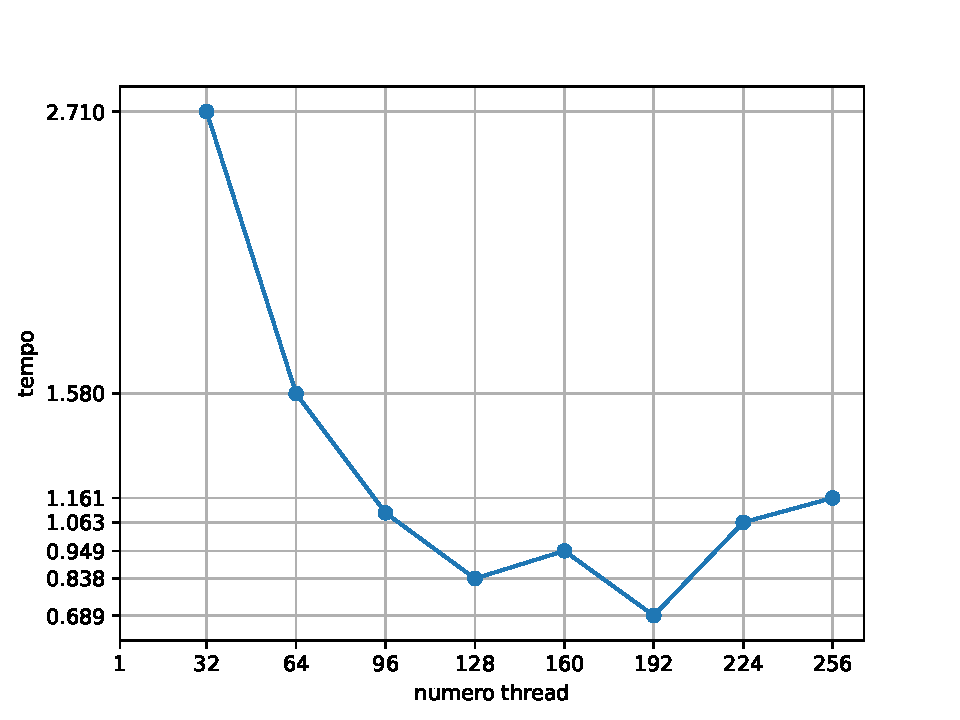
\includegraphics{images/tempi_MPI.pdf}
In seguito è riportato anche il grafico dello speedup degli stessi test precedenti:
%\includegraphics{images/speed_MPI.pdf}
Se si vogliono consultare le informazioni in maniera più pratica, si può conollare la seguente tabella:








\end{document}